\section{Support Vector Machine (Laura Hofer)}
This part was worked on by Laura Hofer (Matnr: 12120724). 
Apart from Random Forest and K-Means, we decided to investigate the performance of Support Vector Machine (SVM) implementations for intrusion detection. 
The applied methodology is based on \cite{SVM} and \cite{dey2023new} and incorporates a Feature Selection with Random Forest, a hyperparameter optimization with Grid Search based on the studies of Dey et al. \cite{dey2023new} and the SVM implementation for binary and multiclass classification. Due to limitations of resources, the SVM approach is implemented in Kaggle\footnote{\url{https://www.kaggle.com/search}} with GPU power, using the preprocessed dataset from the previous steps to stay consistent with the other approaches. Nevertheless, a modification to the data preprocessing was evaluated to increase the performance.

\subsection{Data Preprocessing}
The data preprocessing is based on the previous steps, where the dataset was cleaned and normalized with SMOTE and a MinMaxScaler. These steps helped to reduce the imbalance of the dataset and to scale the features to a range between 0 and 1 for the binary classification of an attack. This implementation has been derived from \cite{SVM}.

\subsection{Feature Selection with Random Forest}
To reduce the overall complexity in dimensionality, the number of features for the SVM model is reduced with the help of a Random Forest Classifier. The classifier has the ability to rank the most important features to enhance the performance of the prediction model. The feature selection is derived from \cite{dey2023new} and \cite{GeeksForGeeks_RandomForestSelection}.

\nextparagraph
For the binary classification with 250 estimators and a random state of 42, the top 45 features were selected, while for the multiclass classification, the top 50 features are considered for more context. For improving the training, a hardware acceleration for Random Forest is used based on RAPIDS cuML, a accelerated machine learning library developed by NVIDIA \cite{GeeksForGeeks_cuML}. 

\subsection{Binary and Multiclass Classification with Support Vector Machine}
For the classification step, the hardware acceleration is also utilized. Scikit-learn and cumllib both support the binary classification with SVM, while for the multiclass classification, a wrapper is implemented to use the GPU acceleration for a one-vs-rest approach, which can be seen in the following algorithm:

\begin{algorithm}[H]
\caption{Training procedure of the GPU One-vs-Rest SVM wrapper}
\label{alg:ovr_wrapper}
\begin{algorithmic}[1]
\ForAll{classes $c \in \mathcal{C}$}
    \State Generate binary labels for class $c$
    \ForAll{training samples}
        \If{sample belongs to class $c$}
            \State Assign label $1$
        \Else
            \State Assign label $0$
        \EndIf
    \EndFor
    \State Compute the class-weight ratio
    \State Train an SVM classifier for class $c$
    \State Store the trained classifier
\EndFor
\end{algorithmic}
\end{algorithm}

\nextparagraph
To further enhance the performance of the multiclass classification of SVM, the training dataset is modified. Only the different attack classes are considered, while the normal class is removed. This is based on the assumption that the model can learn to differentiate between the different attack classes without the normal class.


\subsection{Hyperparameter Tuning}
Derived from the study of Dey et al. \cite{dey2023new}, the hyperparameter tuning is used to find the best combination of parameters for the SVM model. The parameters considered are the regularization parameter $C$ and the RBF kernel parameter $\gamma$. The value range for $C$ is enlarged to $[50, 100, 150, 200, 250, 300]$ and for $\gamma$ to $[0.5, 1.0, 1.5, 2.0, 2.5, 3.0]$ since the higher values achieved a better performance during the evaluation. The target value for the hyperparameter tuning is the f1-score as it incorporates both precision and recall, which is important for the imbalanced dataset. The data used for the hyperparameter tuning is sampled from the training set with a ratio of 20\%.

\subsection{Metrics and Evaluation}
To evaluate the performance of the SVM with Random Forest feature selection, the following metrics are used: accuracy, precision, recall, f1-score, the false positive rate and the Matthews correlation coefficient (MCC). The MCC is a more reliable metric for imbalanced datasets, as it takes into account true and false positives and negatives. The evaluation is performed on the test set, which was not used during the training or hyperparameter tuning.
For the binary classification with  $C = 250$ and $\gamma = 2.5$, a f1-score of 89,49\% was achieved with an MCC score of 79,88\%. Compared to the original papers on which this approach is based on, the performance is slightly lower, which indicates that the SVM model with Random Forest features selection is not as performative as the Mud Ring Assisted Multilayer Support Vector Machine (M-MultiSVM)) approach. This can be attributed to the simplified optimization and alternative approach to the optimization. Nevertheless, the recall is comparably high with 88\% for the attack class and 95\% for the normal class, which indicates that the model is able to detect most of the attacks. Furthermore, the false positive rate is at 8,33\%, which is a good result for the binary classification. Further evaluation results of the binary classification can be found in Table \ref{tab:svm_results}.

\begin{figure}[H]
    \centering
    \label{tab:svm_results}

    \begin{minipage}{0.48\textwidth}
        \centering
        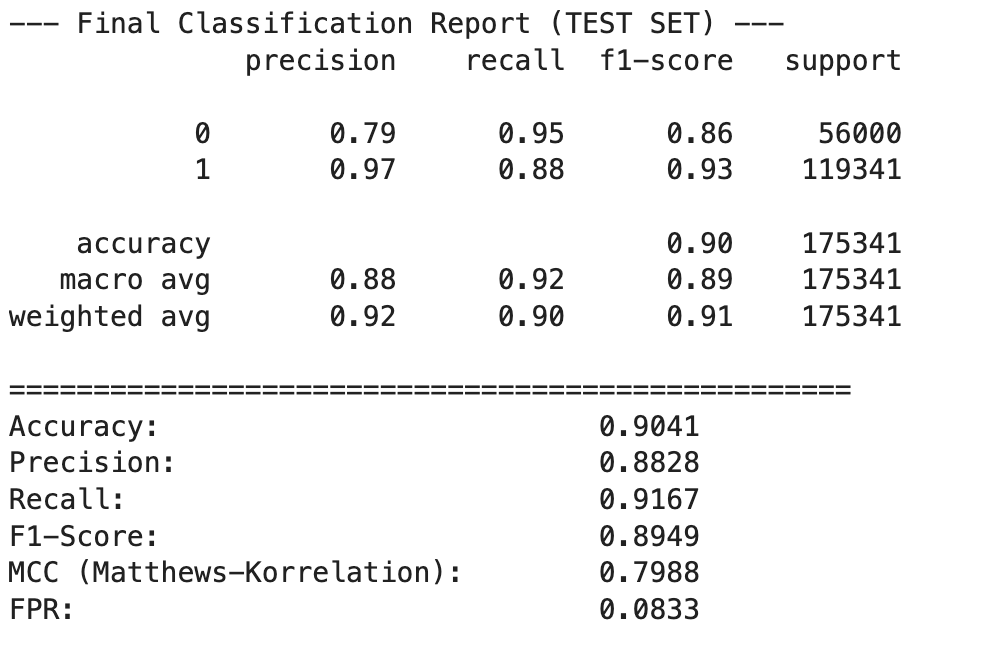
\includegraphics[width=\linewidth]{images/binary_svm.png}
    \end{minipage}
    \hfill
    \begin{minipage}{0.48\textwidth}
        \centering
        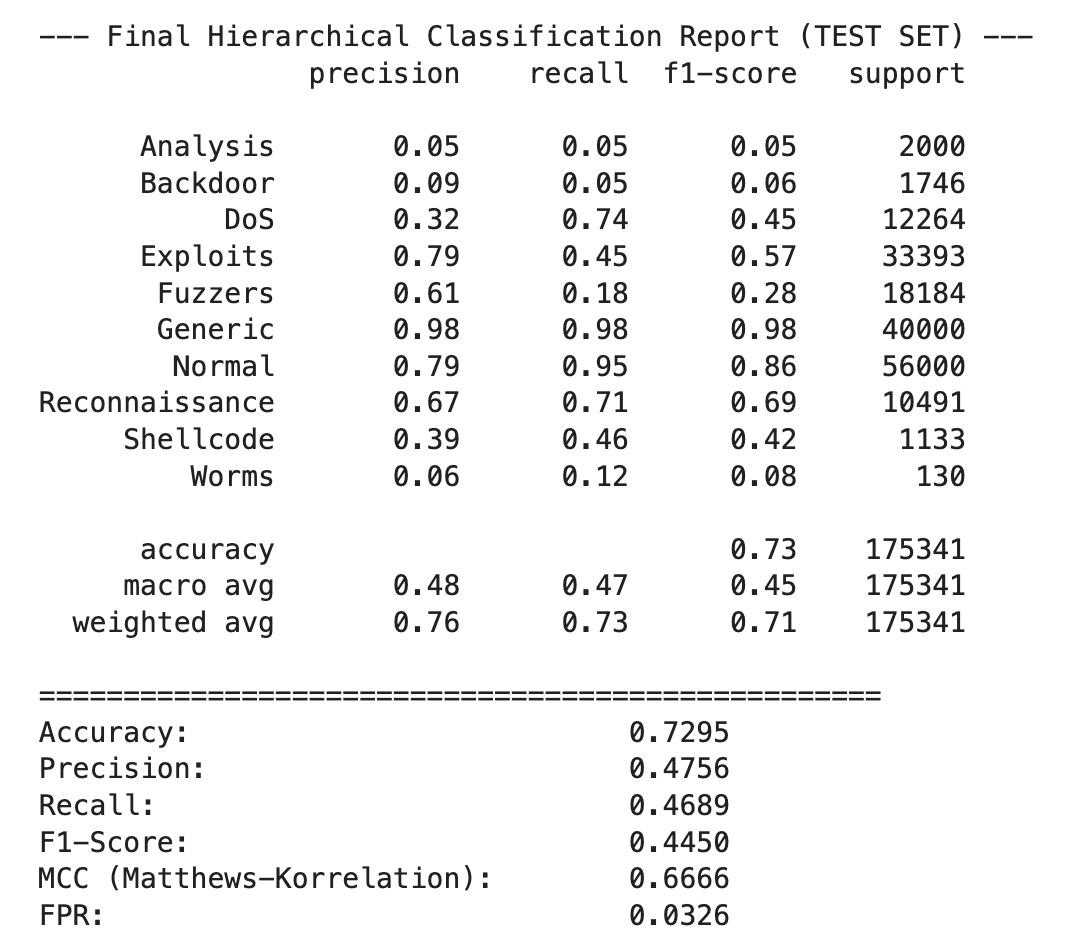
\includegraphics[width=\linewidth]{images/multi_svm.png}
    \end{minipage}
    \caption{Evaluation Results of the Binary and Multiclass Classification of SVM with Random Forest Feature Selection}
\end{figure}

\nextparagraph
The multiclass classification with $C = 250$ and $\gamma = 3.5$ achieved a much lower f1-score of 44,50\% with an MCC score of 66,66\%. The performance is significantly lower compared to the binary classification, which indicates that the SVM model with Random Forest features selection is not able to differentiate between the different attack classes. Nevertheless, the MCC score is comparably high since the false positive rate is at 3,26\%. Especially the worms, analysis and backdoor attacks are not detected well with a f1-score of 8\%, 5\% and 6\%. This can be attributed to the fact that the number of samples for these classes is very low, which makes it difficult for the model to learn the patterns. Further evaluation results of the multiclass classification can be found in Table \ref{tab:svm_results}.